\documentclass[notitlepage]{hw}
\title{Elliptic Functions}
\date{}
\author{}

\usepackage{pgf,tikz}
\usepackage{mathrsfs}
\usetikzlibrary{arrows}

\begin{document}
\maketitle

\section{Introduction}

The Jacobi Elliptic functions come from non-elementary antiderivatives that arise when integrating
over an ellipse. We can define these functions in several ways. One such way is to define the
functions, $sn$, $cn$, and $dn$ as solutions to a system of ordinary differential equations.

\section{Jacobi Functions as solutions to ODEs}

We will begin by making a comparison of JEFs to Trig functions, with which we are familiar. Consider
$\sin{}$ and $\cos{}$. There are many definitions of these two functions, but we will consider a
definition that relates the two functions to ODEs, namely the system
\[
\begin{cases}
\dot{x}=y\\
\dot{y}=-x
\end{cases}.
\]
Under certain initial conditions, this leads to a basis composed of $\sin{}$ and $\cos{}$. It is with
this analogy that we can consider the JEFs.

Suppose we have a system of ODEs as follows
\[
\begin{cases}
\dot{x}=yz\\
\dot{y}=-zx\\
\dot{z}=-k^{2}xy
\end{cases}.
\]
These may seem like arbitrary selections for the system, but, as we will see, they are not. We need
to define $k$ before continuing; it is known as the modulus. We will also want to define the
complimentary modulus, $\kappa=\sqrt{1-k^{2}}$. If we return to our ODEs, we can define the JEFs
as solutions to the system under the following initial conditions:
\[
\begin{cases}
sn(0,k)=x(0)=0\\
cn(0,k)=y(0)=1\\
dn(0,k)=z(0)=1\\
\end{cases}.
\]

We can draw a relationship between $x$, $y$, and $z$ by forming a basis, much like we did with the
ODE definitions of $\sin{}$ and $\cos{}$. Namely, we have that
\[
\{ x,y,z \}\to\{ sn(t,k),cn(t,k),dn(t,k) \}.
\]
This gives rise to the immediate result that
\[
\begin{cases}
{d\over\dt}sn(t,k)=cn(t,k)dn(t,k)\\
{d\over\dt}cn(t,k)=-dn(t,k)sn(t,k)\\
{d\over\dt}dn(t,k)=-k^{2}sn(t,k)cn(t,k)
\end{cases}.
\]

With these properties in mind, we will consider a slightly more geometric view of JEFs.

\section{Jacobi Functions in a Geometric Sense}

We will begin our discussion by considering an ellipse centered about the origin in the cartesian plane.
Such an ellipse can be given by the equation
\[
\left({x^{2}\over a^{2}}\right) + \left({y^{2}\over b^{2}}\right) = 1.
\]
It will benefit us to consider the case where $b=1$, which gives the equation
\[
\left({x^{2}\over a^{2}}\right) + \left(y^{2}\right) = 1.
\]
We can take a given radius $r$ at the point $Q$ on the ellipse, and a given point $P$ at $a$. In
addition, we can call the angle between the the $x$ axis and the radius $\theta$. Rather than consider
a point $(x,y)$, we will actually consider a point $Q=(x(u),y(u))$, where $u$ is a function that we will
define later. We can define the JEFs in terms of this ellipse; we have
\[
\begin{cases}
cn(u,k)=y\\
sn(u,k)={x\over a}\\
dn(u,k)={r\over a}
\end{cases}
\]
\begin{center}
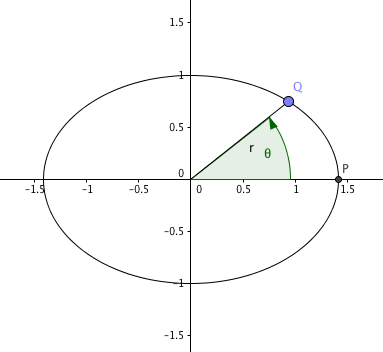
\includegraphics[scale=0.5]{ellipsis}
\end{center}
We can establish some useful identities from this relationship, such as
\[
sn^{2}(u,k)+cn^{2}(u,k)=\left({x\over a}\right)^{2}+y^{2} = 1.
\]
This is similar to our trig identity of $\sin^{2}{x}+\cos^{2}{x}=1$. We also have that
\[
k^{2}sn^{2}(u,k)+dn^{2}(u,k)=1,
\]
which may not be as familiar, but it still holds true. Interestingly enough, we can formulate the
special (or maybe not so special) system of ODEs from the previous section using this new definition.

\section{Jacobi Functions as an Integral}

There is a third definition of JEFs that we can consider; that is, the form they take from an integral.
Consider the ODE
\[
{\dx\over\dt}=\sqrt{(1-x^{2})(1-k^{2}x^{2})}.
\]
We can attempt separation of variables as an approach to solve this. Doing so yields
\[
\int_{0}^{sn(t,k)}{\dx\over\sqrt{(1-x^{2})(1-k^{2}x^{2})}}=t.
\]
The upper limit comes from the comparison to the integral definition of $\sin$:
\[
t=\int_{0}^{\sin{t}}{\dx\over\sqrt{1-x^{2}}}.
\]


\end{document}
